\section{Generation of entangled photons}

Lets consider a nonlinear medium with $\chi_{zzz}^{(2)},\chi_{zyy}^{(2)}\neq0$ and the following Hamiltonian
\begin{align*}
    \hH_{NL}^{(2)}=-\varepsilon_0\int\;dV[\chi_{zzz}^{(2)}E_zE_zE_z+\chi_{zyy}^{(2)}E_zE_yE_y].
\end{align*}

E-field along $z$ and $y$ is:
\begin{align*}
    E_z=\textcolor{Blue}{E_{BZ}}\textcolor{BurntOrange}{\hE_z},\quad\textcolor{BurntOrange}{E_y=\hE_y},\quad\text{where}\quad\begin{array}{l}
        \textcolor{Blue}{\text{Input classical field}}\\
        \textcolor{BurntOrange}{\text{Quantized E-field}}
    \end{array}.
\end{align*}
The first term leads to the Hamiltonian:
\begin{align}
    \hH_{NL,1}^{(2)}=-\frac{3\varepsilon_0}{2}\chi_{zzz}^{(2)}\sqrt{\omega_1\omega_2}(\E_B^*\ha_{1z}\ha^\dagger_{2z}+\E_B\ha_{1z}^\dagger\ha_{2z}^\dagger),\quad\begin{array}{l}
        \omega_1+\omega_2=\omega_B\\
        \bk_1+\bk_2=\bk_B
    \end{array}.
\end{align}
The second term similarly yields 
\begin{align*}
    \hH_{NL,2}^{(2)}=-\varepsilon_0\int\;dV\chi_{zyy}^{(2)}(E_{Bz}+\hE_z)\hE_y\hE_y=-\frac{\varepsilon_0}{2}\chi_{zyy}^{(2)}\sqrt{\omega_1\omega_2}(
        \E_B^\dagger\ha_{1y}\ha_{2y}+\E_B\ha_{1y}^\dagger\ha_{2y}^\dagger),\quad\begin{array}{l}
        \omega_1+\omega_2=\omega_B\\
        \bk_1+\bk_2=\bk_B
    \end{array}.
\end{align*}

Applying the total evolution operator to the vacuum (of all modes):
\begin{align*}
    e^{-i(\hH_{NL,1}^{(2)}+\hH_{NL,2}^{(2)})t/\hbar}\ket{\{0\}}=\ket{\psi_{out}}.
\end{align*}
Assuming that the nonlinearity is weak, we can expand the exponential up to first-order Taylor series:
\begin{align*}
    \ket{\psi_{out}}\approx&\left[\mathds{1}-\frac{it}{\hbar}(\hH_{NL,1}^{(2)}+\hH_{NL,2}^{(2)})\right]\ket{\{0\}}\\
    &\left[\mathds{1}+(\xi_z\ha_{1z}^\dagger\ha_{2z}^\dagger+\xi_z^*\ha_{1z}\ha_{2y})+(\xi_y\ha_{1y}^\dagger\ha_{2y}^\dagger+\xi_y^*\ha_{1y}\ha_{2y})\right]\ket{\{0\}},
\end{align*}
where $\xi_z,\xi_y$ are the squeezing parameters:
\begin{align*}
    \xi_z=-\frac{3i\varepsilon_0t}{2\hbar}\chi_{zzz}^{(2)}\sqrt{\omega_1\omega_2},\quad\xi_y=-\frac{i\varepsilon_0t}{2\hbar}\chi_{zyy}^{(2)}\sqrt{\omega_1\omega_2}.
\end{align*}
Therefore,
\begin{align*}
    \ket{\psi_{out}}\approx\ket{\{0\}}+\xi_z\ket{1}_{1z}\ket{1}_{2z}+\xi_y\ket{1}_{1y}\ket{1}_{2y}.
\end{align*}
Normalizing the above state, assuming that $\xi_z=\xi_y$ and assuming measurement when there is a single photon present in the output:
\begin{align}
    \text{Bell state}\qquad\ket{\psi_{out}}\approx\frac{1}{\sqrt{2}}(\ket{1}_{1z}\ket{1}_{2z}+\ket{1}_{1y}\ket{1}_{2y})\Longleftrightarrow
    \frac{1}{\sqrt{2}}(\ket{z}_{\uparrow}\ket{z}_{\downarrow}+\ket{y}_{\uparrow}\ket{y}_{\downarrow}).
\end{align}


\begin{example}{Four-wave mixing}
    Consider a third-order nonlinear medium with induced nonlinear polarization $\hP_i^{NL}=\varepsilon_0\chi_{ijkl}^{(3)}\hE_j\hE_k\hE_l$.
    Consider that $\chi_{zzzz}\neq0$.
    \begin{enumerate}[itemsep=0pt,topsep=0pt,parsep=0pt,label=\alph*)]
        \item Consider a green laser incident on such a medium. The nonlinearity of the medium can lead to a process where two green photons can 
        combine to generate a pair of entangled red and blue photons. Simplify the following nonlinear Hamiltonian to obtain the energy and momentum 
        conservation conditions 
        \begin{align*}
            \hH_{NL}^{(3)}=-\int_V\;dV\varepsilon_0\chi_{zzzz}^{(3)}\textcolor{Green}{\hE_z}\textcolor{Green}{\hE_z}\textcolor{Red}{\hE_z}\textcolor{Blue}{\hE_z}.
        \end{align*}
        The E-field of the green laser is $\textcolor{Green}{\hE_z}=\hz[\E_Ge^{i(kx-\omega_Gt)}+\E^*_Ge^{-i(kx-\omega_Gt)}]$.
        \item What is the output state for the red and blue modes, considering that the ini-
        tial state of the field in all modes other than the pump is in vacuum and the
        nonlinearity is weak?
        \item onsidering a nonlinear medium with nonzero ($\chi_{zzzz}^{(3)},\chi_{zzyy}^{(3)}\neq0$) ,using the simplified Hamiltonian from part (a), show that four-wave mixing can
        generate two polarization entangled photons.
    \end{enumerate}
    \subsubsection{Solution}
\begin{enumerate}[itemsep=0pt,topsep=0pt,parsep=0pt,label=\alph*)]
  \item Assuming a green laser that combine to generate a pair of entangled red and blue photons. 
  The E-field and operators are:
  \begin{align*}
    \textcolor{Green}{\bE_z}&=\hz\left[\E_Ge^{i(kx-\omega_Gt)}+\E_G^*e^{-i(kx-\omega_Gt)}\right],\\
    \textcolor{BrickRed}{\hbE_z}&=i\sum_{\bk_R}\sqrt{\frac{\hbar\omega_R}{2\varepsilon_0V}}\left[\ha_{\bk_R,z}e^{i(\bk_R\cdot\br-\omega_Rt)}-\ha^\dagger_{\bk_R,z}e^{-i(\bk_R\cdot\br-\omega_R t)}\right],\\
    \textcolor{Blue}{\hbE_z}&=i\sum_{\bk_B}\sqrt{\frac{\hbar\omega_B}{2\varepsilon_0V}}\left[\ha_{\bk_B,z}e^{i(\bk_B\cdot\br-\omega_Bt)}-\ha^\dagger_{\bk_B,z}e^{-i(\bk_B\cdot\br-\omega_Bt)}\right].
  \end{align*}
  Using these definitions in the product integrand of the Hamiltonian yields
  {\small
  \begin{align*}
    \textcolor{Green}{\bE_z}\textcolor{Green}{\bE_z}\textcolor{BrickRed}{\hbE_z}
    \textcolor{Blue}{\hbE_z}=&-\frac{\hbar}{2\varepsilon_0V}\hz\cdot\hz\sum_{\bk_B,\bk_R}\sqrt{\omega_R\omega_B}\left[\E_Ge^{i(kx-\omega_Gt)}+\E_G^*e^{-i(kx-\omega_Gt)}\right]\left[\E_Ge^{i(kx-\omega_Gt)}+\E_G^*e^{-i(kx-\omega_Gt)}\right]\\
    &\left[\ha_{\bk_R,z}e^{i(\bk_R\cdot\br-\omega_Rt)}-\ha^\dagger_{\bk_R,z}e^{-i(\bk_R\cdot\br-\omega_R t)}\right]
    \left[\ha_{\bk_B,z}e^{i(\bk_B\cdot\br-\omega_Bt)}-\ha^\dagger_{\bk_B,z}e^{-i(\bk_B\cdot\br-\omega_Bt)}\right].
  \end{align*}}
  By distributing all the terms above, we will have different combinations of frequency and wavevectors.
  In particular,
  \begin{align*}
    \omega:\;e^{i(\pm 2\omega_G\pm\omega_R\pm\omega_B)t}\quad\land\quad\bk:\;e^{i[\pm2kx+(\pm\bk_R\pm\bk_B)\cdot\br]}.
  \end{align*}
  The only terms that are slow oscillating are the ones that are nearly zero, obtaining the energy and 
  momentum conservation:
  \begin{align*}
    \pm2\omega_G\mp(\omega_R+\omega_B)=0&\Longrightarrow\text{Energy conservation}:2\omega_G=\omega_R+\omega_B,\\
    \pm2kx\mp(\bk_R+\bk_B)&\Longrightarrow\text{Momentum conservation}:2kx=\bk_R+\bk_B.
  \end{align*}
  The difference of blue and red frequencies is still in the optical frequency. The Hamiltonian then reduces to
  \begin{align*}
    \hH_{NL,1}^{(3)}=\frac{\hbar\sqrt{\omega_R\omega_B}}{2}\chi_{zzzz}^{(3)}\left[\E_G^2\ha^\dagger_{\bk_R,z}\ha^\dagger_{\bk_B,z}+\E_G^{*2}\ha_{\bk_R,z}\ha_{\bk_B,z}\right]. 
  \end{align*}
  \item The evolution operator applied to the vaccum state of R and B light $\ket{0}_R\ket{0}_B=\ket{\{0\}}$ is:
  \begin{align*}
    \hU(t,0)=e^{-i\hH_{NL,1}^{(3)}t/\hbar}\ket{\{0\}}=e^{-i\left\{\frac{\hbar\sqrt{\omega_R\omega_B}}{2}\chi_{zzzz}^{(3)}\left[\E_G^2\ha^\dagger_{\bk_R,z}\ha^\dagger_{\bk_B,z}+\E_G^{*2}\ha_{\bk_R,z}\ha_{\bk_B,z}\right]\right\}t/\hbar}=\ket{\psi_{out}}
  \end{align*}
  Expanding the exponential to the first-order Taylor series yields:
  \begin{align*}
    \left\{\mathds{1}-i\frac{\sqrt{\omega_R\omega_B}\chi_{zzzz}^{(3)}}{2}\left[\E_G^2\ha^\dagger_{\bk_R,z}\ha^\dagger_{\bk_B,z}+\E_G^{*2}\ha_{\bk_R,z}\ha_{\bk_B,z}\right]t\right\}\ket{\{0\}}.
  \end{align*}
  By defining the squeezing parameter $\xi_z$ as:
  \begin{align*}
    \xi_z=-i\frac{\sqrt{\omega_R\omega_B}\chi_{zzzz}^{(3)}}{2}\E_G^2t,
  \end{align*}
  we have:
  \begin{align*}
    \left[\mathds{1}+\xi_z\ha^\dagger_{\bk_R,z}\ha^\dagger_{\bk_B,z}+\xi^*_z\ha_{\bk_R,z}\ha_{\bk_B,z}\right]\ket{\{0\}}=\ket{\{0\}}+\xi_z\ket{1}_{R_z}\ket{1}_{B_z}.
  \end{align*}
  \item The process for the new term is esentially the same, with the change of 
  the last two indices to y polarization. The Hamiltonian for this term 
  is: 
  \begin{align*}
    \hH^{(3)}_{NL,2}=\frac{\hbar\sqrt{\omega_R\omega_B}}{2}\chi_{zzyy}^{(3)}\left[\E^2_G\ha^\dagger_{\bk_R,y}\ha^\dagger_{\bk_B,y}+\E^{*2}_G\ha_{\bk_R,y}\ha_{\bk_B,y}\right]
  \end{align*}
  The total Hamiltonian is the sum of the individual Hamiltonian:
  \begin{align*}
    \hH_{NL}^{(3)}&=\hH_{NL,1}^{(3)}+\hH_{NL,2}^{(3)}\\
    \hH_{NL}^{(3)}&=\frac{\hbar\sqrt{\omega_R\omega_B}}{2}\left[\chi_{zzzz}^{(3)}\E_G^2\ha^\dagger_{\bk_R,z}\ha^\dagger_{\bk_B,z}+\E^{*2}_G\ha_{\bk_R,z}\ha_{\bk_B,z}+
    \chi_{zzyy}^{(3)}\E_G^2\ha^\dagger_{\bk_R,y}\ha^\dagger_{\bk_B,y}+\E^{*2}_G\ha_{\bk_R,y}\ha_{\bk_B,y}\right].
  \end{align*}
  The first-order Taylor expansion of the evolution operator is:
  \begin{align*}
    U(t,0)=e^{-i\hN_{NL}^{(3)}t/\hbar}\approx\mathds{1}+\xi_z\ha^\dagger_{\bk_R,z}\ha^\dagger_{\bk_B,z}+\xi^*_z\ha_{\bk_R,z}\ha_{\bk_B,z}+\xi_y\ha^\dagger_{\bk_R,y}\ha^\dagger_{\bk_B,y}+\xi^*_y\ha_{\bk_R,y}\ha_{\bk_B,y},
  \end{align*}
  where the squeezing parameters are:
  \begin{align*}
    \xi_z=-i\frac{\sqrt{\omega_R\omega_B}\chi_{zzzz}^{(3)}}{2}\E_G^2t,\quad\text{and}\quad\xi_y=-i\frac{\sqrt{\omega_R\omega_B}\chi_{zzyy}^{(3)}}{2}\E_G^2t.
  \end{align*}
  Application of the evolution operator in the vaccum state produces:
  {\small
  \begin{align*}
    \left[\mathds{1}+\xi_z\ha^\dagger_{\bk_R,z}\ha^\dagger_{\bk_B,z}+\xi^*_z\ha_{\bk_R,z}\ha_{\bk_B,z}+\xi_y\ha^\dagger_{\bk_R,y}\ha^\dagger_{\bk_B,y}+\xi^*_y\ha_{\bk_R,y}\ha_{\bk_B,y}\right]\ket{\{0\}}=\ket{\{0\}}+\xi_z\ket{1}_{R_z}\ket{1}_{B_z}+\xi_y\ket{1}_{R_y}\ket{1}_{B_y}.
  \end{align*}}
  Generating in that way, two polarization entangled photons.
\end{enumerate}
\end{example}

\begin{example}{Entangled photons through a BS}
  Consider the following setup.
  \begin{figure}[htbp]
    \centering
    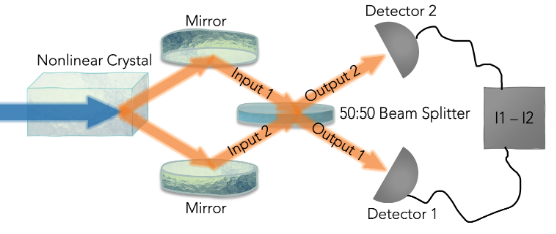
\includegraphics[width=.4\columnwidth]{PartOne/ChapterThree/figures/hongoumandelsetup.png}
  \end{figure}
  
  The state of the two photons exiting the nonlinear crystal is: i) $\ket{1}_1\ket{1}_2$, ii) $\frac{1}{\sqrt{2}}(\ket{1}_1\ket{0}_2+\ket{0}_1\ket{1}_2)$, 
  and iii) $\frac{1}{\sqrt{2}}(\ket{1}_1\ket{0}_2-\ket{0}_1\ket{1}_2)$. Find $\braket{\hI_k}$ and $\braket{\hI_1-\hI_2}$.
  \subsubsection{Solution}
  The intensity operator for each detector and the difference is:
  \begin{align*}
    \hI_1&=\hb_1^\dagger\hb_1=\frac{1}{2}(\ha_1^\dagger+\ha^\dagger_2)(\ha_1+\ha_2)=\frac{1}{2}(\ha_1^\dagger\ha_1+\ha_1^\dagger\ha_2+\ha_2^\dagger\ha_1+\ha_2^\dagger\ha_2),\\
    \hI_2&=\hb_2^\dagger\hb_2=\frac{1}{2}(\ha_1^\dagger-\ha^\dagger_2)(\ha_1-\ha_2)=\frac{1}{2}(\ha_1^\dagger\ha_1-\ha_1^\dagger\ha_2-\ha_2^\dagger\ha_1+\ha_2^\dagger\ha_2),\\
    \hI_1-\hI_2&=\ha_1^\dagger\ha_2+\ha_2^\dagger\ha_1.
  \end{align*}
  We use these to compute the expected number of photons $\braket{\hI_k}$ at individual detectors and the difference $\braket{\hI_1-\hI_2}$.
  \begin{enumerate}[itemsep=0pt,topsep=0pt,parsep=0pt,label=\roman*)]
    \item 
    \begin{align*}
      \braket{\hI_1}&=\frac{1}{2}\braket{1,1|(\ha_1^\dagger\ha_1+\ha_1^\dagger\ha_2+\ha_2^\dagger\ha_1+\ha_2^\dagger\ha_2)|1,1}=1,\\
      \braket{\hI_2}&=\frac{1}{2}\braket{1,1|(\ha_1^\dagger\ha_1-\ha_1^\dagger\ha_2-\ha_2^\dagger\ha_1+\ha_2^\dagger\ha_2)|1,1}=1,\\
      \braket{\hI_1-\hI_2}&=0.
    \end{align*}
    \item In this case of entangled photons, we follow the definition of the expected value and we use distribution property:
    {\small
    \begin{align*}
      \braket{\hI_1}=\left[\frac{1}{\sqrt{2}}(\bra{0,1}+\bra{1,0})\right]|\hb_1^\dagger\hb_1|\left[\frac{1}{\sqrt{2}}(\ket{1,0}+\ket{0,1})\right]=\frac{1}{4}(\bra{0,1}+\bra{1,0})|(\ha_1^\dagger\ha_1+\ha_1^\dagger\ha_2+\ha_2^\dagger\ha_1+\ha_2^\dagger\ha_2)|(\ket{1,0}+\ket{0,1}).
    \end{align*}}
    I should distribute and solve the 16 terms. However, I can express the input in the following way:
    \begin{align*}
      \ket{\psi}=\frac{1}{\sqrt{2}}(\ha_1^\dagger+\ha_2^\dagger)\ket{0,0}=\hb_1^\dagger\ket{0,0}=\ket{1',0'}.
    \end{align*}
    which is simpler to use, because:
    \begin{align*}
      \braket{\hI_1}=\braket{0',1'|\hb_1^\dagger\hb_1|1',0'}=\braket{0',1'|1',0'}=1.
    \end{align*}
    For the detector 2, the expected number of photon is:
    \begin{align*}
      \braket{\hI_2}=\braket{0',1'|\hb_2^\dagger\hb_2|1',0'}=0.
    \end{align*}
    Therefore,
    \begin{align*}
      \braket{\hI_1-\hI_2}=\braket{\hI_1}-\braket{\hI_2}=1.
    \end{align*}
    \item Using the form from previous part, the entangled state is:
    \begin{align*}
      \ket{\psi}=\frac{1}{\sqrt{2}}(\ket{1,0}-\ket{0,1})=\frac{1}{\sqrt{2}}(\ha_1^\dagger-\ha_2^\dagger)\ket{0,0}=\hb_2^\dagger\ket{0,0}=\ket{0',1'}.
    \end{align*}
    Now, 
    \begin{align*}
      \braket{\hI_1}&=\braket{0',1'|\hb_1^\dagger\hb_2'|1',0'}=0,\\
      \braket{\hI_2}&=\braket{0',1'|\hb_2^\dagger\hb_2|0',1'}=1,\\
      \braket{\hI_1-\hI_2}&=-1.
    \end{align*}
  \end{enumerate}
\end{example}

